%%%%%%%%%%%%%%%%%%%%%%%%%%%%%%%%%%%%%%%%%%%%%%%%%%%%%%%%%%%
% --------------------------------------------------------
% Tau
% LaTeX Template
% Version 2.4.4 (28/02/2025)
%
% Author: 
% Guillermo Jimenez (memo.notess1@gmail.com)
% 
% License:
% Creative Commons CC BY 4.0
% --------------------------------------------------------
%%%%%%%%%%%%%%%%%%%%%%%%%%%%%%%%%%%%%%%%%%%%%%%%%%%%%%%%%%%

%\documentclass[9pt,a4paper,twocolumn,twoside]{tau-class/tau}
%\usepackage[english]{babel}
%\usepackage{indentfirst} % 添加这个宏包使每个段落的第一行缩进
%%% Spanish babel recomendation
% \usepackage[spanish,es-nodecimaldot,es-noindentfirst]{babel} 

%% Draft watermark
% \usepackage{draftwatermark}

%----------------------------------------------------------
% TITLE
%----------------------------------------------------------
\setcounter{section}{0}
\journalname{2025 - Control Engineering Practice - Article 3}
\title{An integrated framework for motion planning and trajectory optimization of AGVs using spatio-temporal safety corridors}

%----------------------------------------------------------
% AUTHORS, AFFILIATIONS AND PROFESSOR
%----------------------------------------------------------

\author{Xi Zhang, Yaomin Lu,Zhiyang Ju}
%\author{Marios Spanakakis}
%\author{Johannes Betz}

%%----------------------------------------------------------
%
%\affil[a]{Affiliation of author one}
%\affil[b]{Affiliation of author two}
%\affil[c]{Affiliation of author three}

%\professor{Professor/Authority or other information}

%----------------------------------------------------------
% FOOTER INFORMATION
%----------------------------------------------------------
%
%\institution{College name}
%\footinfo{\LaTeX\ Template}
%\theday{July 26, 2024}
%\leadauthor{Author last name et al.}
%\course{Creative Commons CC BY 4.0}

%----------------------------------------------------------
% ABSTRACT AND KEYWORDS
%----------------------------------------------------------
\maketitle
\section{Abstract} 
Efficiently generating safe and smooth trajectories for autonomous ground vehicles (AGVs) is a crucial and challenging task, particularly in dynamic environments with moving obstacles. This paper proposes an integrated motion planning and trajectory optimization (MPTO) framework that employs an optimization-based spatio-temporal safety corridors (STSC) to ensure trajectory smoothness and safety from a three-dimensional spatio-temporal perspective. The proposed MPTO framework comprises two layers. In the first layer, a multi-objective quadratic programming (MOQP) method was developed with the objective of rapidly generating smoothly varying STSC. The multi-objective cost function provides a comprehensive evaluation of the corridors in terms of their size, direction, and smoothness. Additionally, a convex polygonal feasible area (CPFA) was proposed to provide a linear obstacle-avoidance constraint for the MOQP. The smooth STSC provides within-corridor constraints for trajectory optimization, thereby ensuring collision avoidance of obstacles and reducing the dependence of trajectory optimization on the reference trajectory. In the second layer, an optimal trajectory generation method using polynomials is proposed to generate smooth and efficient trajectories. With smooth STSC constraints, the trajectory optimization model primarily focuses on smoothness, ensuring that the trajectory remains safe and smooth even with sudden changes in the feasible area. Finally, the proposed MPTO framework is validated through simulations and real vehicle experiments.

%----------------------------------------------------------

%\keywords{\LaTeX\ class, lab report, academic article, tau class}

%----------------------------------------------------------

%\begin{document}
%		
%    \maketitle 
%    \thispagestyle{firststyle} 
%    \tauabstract 
    % \tableofcontents
    % \linenumbers 
    
%----------------------------------------------------------

\section{Contextual Challenges Introduction}
The complexity of generating safe and smooth trajectories for Automated Ground Vehicles (AGVs) in dynamic environments arises from the presence of moving obstacles. Path planning must consider not only spatial dimensions but also the temporal aspect, making trajectory planning significantly more complex than path planning. Additionally, the dynamic changes in feasible areas have a significant impact on safety, requiring a balance between safety and smoothness. Although high-quality reference trajectories or larger safety thresholds can address this issue, they lead to increased time consumption or reduced free space. Therefore, the authors emphasize the necessity of developing theoretically sound frameworks to ensure the smoothness and safety of AGV paths in three-dimensional space-time without adding extra complexity.
\section{Related Works}
In this article, previous work is summarized into three approaches: search-based methods, optimization-based methods, and two-stage methods.
\subsection{Search-Based Methods}
Advantages: These methods can easily handle constraints in high-dimensional configuration spaces. The basic idea is to discretize the continuous space and then apply algorithms on the discretized data to find the optimal solution. This approach is naturally suited for high-dimensional constraint problems and is insensitive to the complexity of constraints. However, it faces challenges related to time consumption and trajectory quality.
\subsection{Optimization-Based Methods}
Advantages: These methods solve problems in continuous space and are advantageous for generating high-precision trajectories. The basic idea is to describe the trajectory planning problem as an optimization problem, defining objective functions and constraints to achieve high-precision trajectories. However, the computational complexity is high, especially when dealing with non-convex constraints, which can easily lead to local optima.
\subsection{Two-Stage Methods}
Stage 1: Use search-based methods to identify the most promising homotopy class paths globally. Stage 2: Use optimization-based methods to find a local optimal solution. This approach combines global path planning with local path adjustment but may lead to drastic changes in the global path, affecting vehicle safety and comfort. 

\textbf{Summary:} By introducing additional safety constraints, path changes can be somewhat suppressed; however, the aforementioned methods increase computational costs and restrict the vehicle's driving space.

\section{Proposed Work}

1.Proposed MPTO Framework (Motion Planning and Trajectory Optimization)

This framework includes two lightweight optimization models: one for motion planning and one for trajectory optimization. It ensures that the process of generating spatio-temporal trajectories is efficient, resulting in paths that are both safe and smooth.

2.Proposed STSC Framework (Spatio-Temporal Safety Corridor)

This framework effectively addresses the collision-prone issues of traditional corridors. By dynamically adjusting corridors, optimizing space, and designing reference trajectory deviation penalties, STSC flexibly generates freer and safer corridors. Note: A corridor refers to the potential area where a driving path may be laid out, acting as a safety channel. It is designed to ensure that paths within this range are considered safe. The workflow of this paper follows the approach of "corridor generation → path generation → corridor adjustment → path constraint."

3.Conducted Simulations and Real-World Tests

The effectiveness and practicality of the proposed MPTO method were validated through simulations and real vehicle experiments.
\section{My Perspective on This Paper}
The article addresses the issue of increased computational costs and reduced path freedom due to safety constraints, proposing a framework that maintains low overall costs, high reliability, and generates smooth paths. The transition from previous research achievements to the author's own findings is seamless, similar to what is seen in article 1, making it a valuable point of study. Additionally, the article features excellent illustrations, particularly the following two figures. Figure 1 describes the process of corridor generation and optimization, while Figure 2 showcases the safety performance of different RL methods. Both are aesthetically pleasing and intuitive.
    	\begin{figure}[H]
    		\centering
    		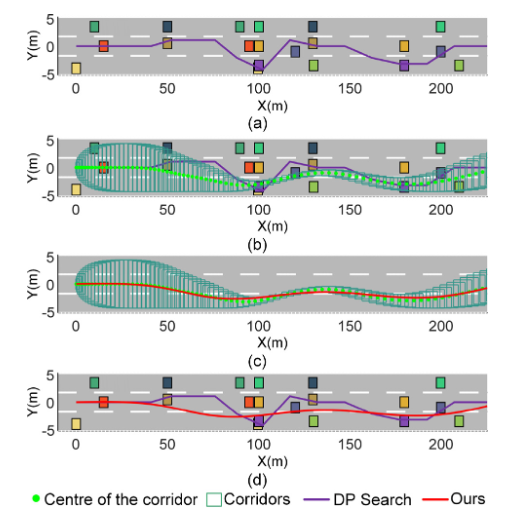
\includegraphics[width=0.75\columnwidth]{F1.png}
    		\caption{The process of corridor generation and optimization.}
    		\label{fig:figure}
    	\end{figure}
    	\begin{figure}[H]
    		\centering
    		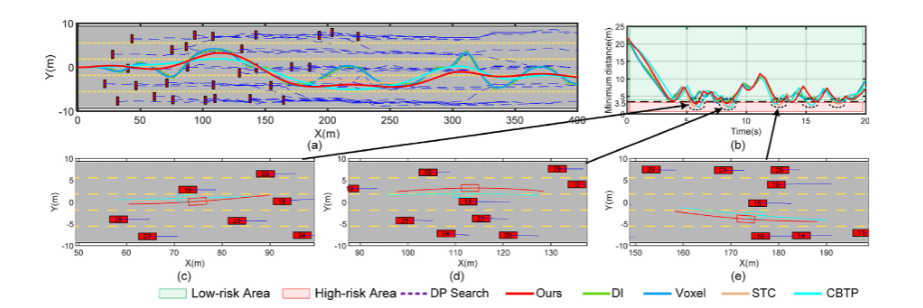
\includegraphics[width=0.75\columnwidth]{F2.png}
    		\caption{The safety performance of different RL methods.}
    		\label{fig:figure}
    	\end{figure}

%----------------------------------------------------------- 第3篇文章结束 ---------------------------------------------------------------
%----------------------------------------------------------
%
%\printbibliography
%----------------------------------------------------------
%
%\end{document}